
\documentclass[a4paper,11pt]{article}
\usepackage[a4paper, margin=8em]{geometry}

% usa i pacchetti per la scrittura in italiano
\usepackage[french,italian]{babel}
\usepackage[T1]{fontenc}
\usepackage[utf8]{inputenc}
\frenchspacing 

% usa i pacchetti per la formattazione matematica
\usepackage{amsmath, amssymb, amsthm, amsfonts}

% usa altri pacchetti
\usepackage{gensymb}
\usepackage{hyperref}
\usepackage{standalone}

% imposta il titolo
\title{Appunti Elettronica Digitale}
\author{Luca Seggiani}
\date{2026}

% imposta lo stile
% usa helvetica
\usepackage[scaled]{helvet}
% usa palatino
\usepackage{palatino}
% usa un font monospazio guardabile
\usepackage{lmodern}

\renewcommand{\rmdefault}{ppl}
\renewcommand{\sfdefault}{phv}
\renewcommand{\ttdefault}{lmtt}

% disponi il titolo
\makeatletter
\renewcommand{\maketitle} {
	\begin{center} 
		\begin{minipage}[t]{.8\textwidth}
			\textsf{\huge\bfseries \@title} 
		\end{minipage}%
		\begin{minipage}[t]{.2\textwidth}
			\raggedleft \vspace{-1.65em}
			\textsf{\small \@author} \vfill
			\textsf{\small \@date}
		\end{minipage}
		\par
	\end{center}

	\thispagestyle{empty}
	\pagestyle{fancy}
}
\makeatother

% disponi teoremi
\usepackage{tcolorbox}
\newtcolorbox[auto counter, number within=section]{theorem}[2][]{%
	colback=blue!10, 
	colframe=blue!40!black, 
	sharp corners=northwest,
	fonttitle=\sffamily\bfseries, 
	title=~\thetcbcounter: #2, 
	#1
}

% disponi definizioni
\newtcolorbox[auto counter, number within=section]{definition}[2][]{%
	colback=red!10,
	colframe=red!40!black,
	sharp corners=northwest,
	fonttitle=\sffamily\bfseries,
	title=~\thetcbcounter: #2,
	#1
}

% U.D.M
\newcommand{\amp}{\ensuremath{\mathrm{A}}}
\newcommand{\volt}{\ensuremath{\mathrm{V}}}
\newcommand{\meter}{\ensuremath{\mathrm{m}}}
\newcommand{\second}{\ensuremath{\mathrm{s}}}
\newcommand{\farad}{\ensuremath{\mathrm{F}}}
\newcommand{\henry}{\ensuremath{\mathrm{H}}}
\newcommand{\siemens}{\ensuremath{\mathrm{S}}}

% circuiti
\usepackage{circuitikz}
\usetikzlibrary{babel}

% disegni
\usepackage{pgfplots}
\pgfplotsset{width=10cm,compat=1.9}

% disponi codice
\usepackage{listings}
\usepackage[table]{xcolor}

\definecolor{codegreen}{rgb}{0,0.6,0}
\definecolor{codegray}{rgb}{0.5,0.5,0.5}
\definecolor{codepurple}{rgb}{0.58,0,0.82}
\definecolor{backcolour}{rgb}{0.95,0.95,0.92}

\lstdefinestyle{codestyle}{
		backgroundcolor=\color{black!5}, 
		commentstyle=\color{codegreen},
		keywordstyle=\bfseries\color{magenta},
		numberstyle=\sffamily\tiny\color{black!60},
		stringstyle=\color{green!50!black},
		basicstyle=\ttfamily\footnotesize,
		breakatwhitespace=false,         
		breaklines=true,                 
		captionpos=b,                    
		keepspaces=true,                 
		numbers=left,                    
		numbersep=5pt,                  
		showspaces=false,                
		showstringspaces=false,
		showtabs=false,                  
		tabsize=2
}

\lstdefinestyle{shellstyle}{
		backgroundcolor=\color{black!5}, 
		basicstyle=\ttfamily\footnotesize\color{black}, 
		commentstyle=\color{black}, 
		keywordstyle=\color{black},
		numberstyle=\color{black!5},
		stringstyle=\color{black}, 
		showspaces=false,
		showstringspaces=false, 
		showtabs=false, 
		tabsize=2, 
		numbers=none, 
		breaklines=true
}

\lstdefinelanguage{javascript}{
	keywords={typeof, new, true, false, catch, function, return, null, catch, switch, var, if, in, while, do, else, case, break},
	keywordstyle=\color{blue}\bfseries,
	ndkeywords={class, export, boolean, throw, implements, import, this},
	ndkeywordstyle=\color{darkgray}\bfseries,
	identifierstyle=\color{black},
	sensitive=false,
	comment=[l]{//},
	morecomment=[s]{/*}{*/},
	commentstyle=\color{purple}\ttfamily,
	stringstyle=\color{red}\ttfamily,
	morestring=[b]',
	morestring=[b]"
}

% disponi sezioni
\usepackage{titlesec}

\titleformat{\section}
	{\sffamily\Large\bfseries} 
	{\thesection}{1em}{} 
\titleformat{\subsection}
	{\sffamily\large\bfseries}   
	{\thesubsection}{1em}{} 
\titleformat{\subsubsection}
	{\sffamily\normalsize\bfseries} 
	{\thesubsubsection}{1em}{}

% disponi alberi
\usepackage{forest}

\forestset{
	rectstyle/.style={
		for tree={rectangle,draw,font=\large\sffamily}
	},
	roundstyle/.style={
		for tree={circle,draw,font=\large}
	}
}

% disponi algoritmi
\usepackage{algorithm}
\usepackage{algorithmic}
\makeatletter
\renewcommand{\ALG@name}{Algoritmo}
\makeatother

% disponi numeri di pagina
\usepackage{fancyhdr}
\fancyhf{} 
\fancyfoot[L]{\sffamily{\thepage}}

\makeatletter
\fancyhead[L]{\raisebox{1ex}[0pt][0pt]{\sffamily{\@title \ \@date}}} 
\fancyhead[R]{\raisebox{1ex}[0pt][0pt]{\sffamily{\@author}}}
\makeatother

\begin{document}
% sezione (data)
\section{Lezione del 14-04-26}

% stili pagina
\thispagestyle{empty}
\pagestyle{fancy}

% testo
Abbiamo visto nella scorsa lezione la struttura del transistore di tipo \textbf{MOSFET} (\textit{Metal Oxide Semiconductor Field Effect Transistor}). Andiamo adesso a vedere quella che è la \textit{caratteristica di funzionamento}.

Le ipotesi che avevamo fatto erano:
\begin{enumerate}
	\item Lo strato di ossido è perfetto, cioè non si ha mai conduzione di corrente dal gate:
		$$
		I_G = 0
		$$
	\item Le giunzioni drain-body e source-body sono polarizzate in inversa, per cui si comportano come diodi e non esiste corrente di corpo:
		$$
		I_B = 0
		$$
\end{enumerate}

Vediamo quindi il funzionamento del MOSFET in diverse zone di operazione:
\begin{itemize}
\item $V_B = 0$, $V_S = 0$, $V_D = 0$, $V_G > 0$ \\
In questo caso tutti i morsetti sono a massa tranne il gate, a cui imponiamo una certa tensione.

Possiamo suddividere ulteriormente questa zona in:
\begin{itemize}
\item $V_G$ positiva e molto piccola ($V_G << V_T$ tensione di soglia): in questo caso tra source e drain non c'è alcun percorso chiuso. Per spiegarci come mai, vediamo che attorno alle regioni drogate $N^+$ del substrato si vanno a formare zone di svuotamento, con ioni fissi positivi all'interno della zona $N^+$, e ioni fissi negativi al confine del substrato $P$. 

Con $V_G$ molto minore della tensione di soglia il MOS non è ancora in svuotamento, per cui la situazione è effettivamente invariata (le zone di svuotamento restano legate alle regioni drogate $N^+$);

\item $V_G$ positiva confrontabile a $V_T$ ($V_G > 0$, $V_G < V_T$ tensione di soglia): quando la $V_G$ diventa comparabile con la tensione di soglia si ha che il MOS va in \textit{svuotamento}, per cui ci troviamo nella situazione dove le zone di svuotamento $N^+$, prima separate, si uniscono formando una sorta di "ponte" di ioni negativi fissi;

\item $V_G$ positiiva maggiore di $V_T$ ($V_G > 0$, $V_G > V_T$ tensione di soglia): se la $V_G$ supera la soglia il MOS va a trovarsi in \textit{inversione}, e appena sotto lo strato di ossido si va a formare un sottile strato di cariche negative (stavolta non fisse, ma mobili, cioè rappresentate dagli elettroni liberi, portatori di minoranza, del substrato $P$). 

Grazie alla presenza dei pozzetti $N^+$ a sinistra e a destra del gate, riusciamo a mantenere lo strato per tutta la lunghezza del gate collegando le due regioni $N^+$ (questo era quello che avevamo anticipato studiando il condensatore MOS). Abbiamo quindi messo in comunicazione source e drain, creando un \textit{canale} di conduzione fra di essi.
\end{itemize}

\item $V_B = 0$, $V_S = 0$, $V_D > 0$, $V_G > 0$ \\

Prendiamo quindi il source a 0 come riferimento (il body lo assumeremo sempre a 0), e applichiamo una tensione al gate e al drain.

Vediamo anche qui le suddivisioni:
\begin{itemize}
	\item $V_G$ positiva maggiore di $V_T$, e $V_D$ positiva piccola ($V_G > V_T$, $V_D > 0$): in questo caso chiaramente abbiamo creato il canale di conduzione fra source e drain (dal fatto che $V_G > V_T$ e siamo in inversione del MOS). A questo punto, visto che abbiamo una certa tensione al drain, ci sarà conduzione di elettroni dal source verso il drain e quindi una corrente convenzionale dal drain al source:
	$$
	I_{DS} > 0
	$$

	In prima approssimazione, quindi, il comportamento del MOSFET è lineare sulla tensione al drain, e ad un incremento della tensione applicata si ha un incremento proporzionale della corrente. Incrementando la $V_G$ si ha che la costante di proporzionalità lineare aumenta, anch'essa in maniera pressapoco lineare:
	\begin{center}
		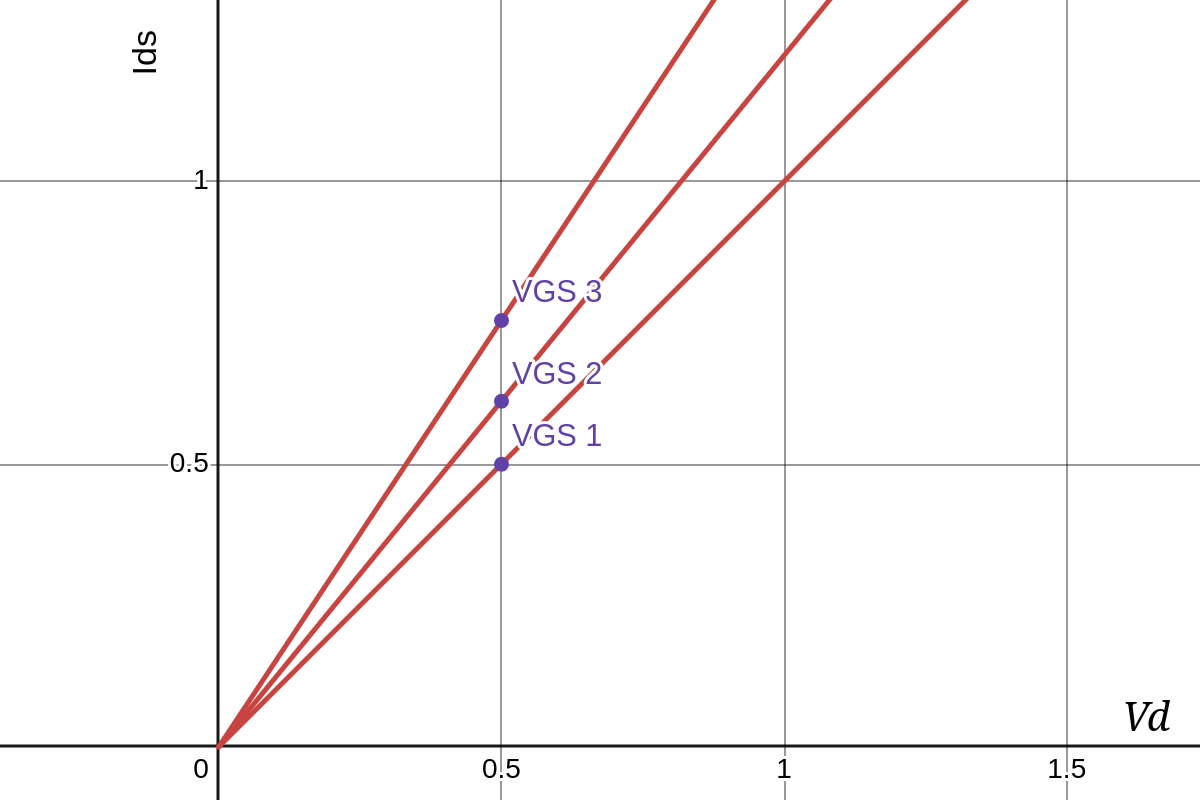
\includegraphics[scale=0.25]{../figures/triode_mode.png}
	\end{center}

	Abbiamo quindi realizzato una resistenza controllata in tensione: per questo motivo il comportamento del MOSFET in questa regione viene detto a \textit{triodo}, o \textbf{ohmico}.

\item $V_G$ positiva maggiore di $V_T$, e $V_D$ positiva ($V_G > V_T$, $V_D > 0$): vediamo cosa accade se si aumenta $V_D$ ulteriormente.

Abbiamo che la tensione lungo il canale di conduzione può essere rappresentata da una funzione $\phi(x)$ campionata da $0$ (al limite del source) a $L$ (al limite del drain) con $L$ larghezza del canale stesso:
$$
\phi(x) = \frac{V_{D}x}{L}, \quad \left\{0\le x\le L\right\}
$$
Sarà che $\phi(x)$ attorno al source (cioè $\phi(0)$) varrà 0, mentre $\phi(x)$ attorno al drain (cioè $\phi(L)$) rispetterà il valore imposto $V_G$. 

Ora, per un qualsiasi punto $x_i$ lungo il canale, essere effettivamente in inversione significa assumere:
$$
V_{Gx_i} \geq V_T, \quad V_{Gx_i} = V_G - V_{x_i} = V_G - \phi(x_i)
$$
cioè che la differenza di potenziale fra il gate e il punto $x_i$ sia maggiore della tensione di soglia.

	\begin{center}
		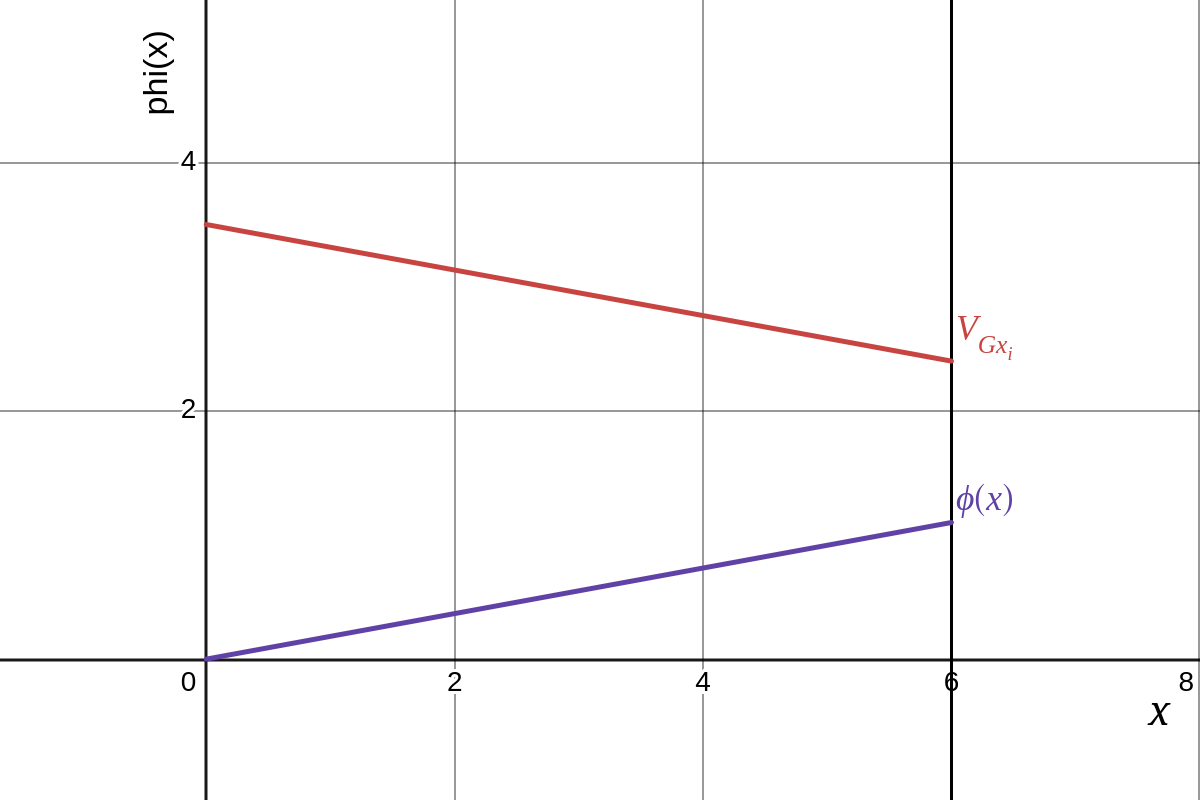
\includegraphics[scale=0.25]{../figures/channel_cond.png}
	\end{center}

Vicino al source, questa $V_{Gx_i}$ sarà circa la tensione di gate:
$$
x_i = 0 \implies V_{G x_i} = V_G
$$
mentre vicino al drain questa diminuirà fino ad un certo valore:
$$
x_i = L \implies V_{G x_i} = V_G - V_D
$$

Avremo quindi una diminuzione della sezione del canale di elettroni formatosi lungo la lunghezza del canale stesso. Essendo questo canale la nostra resistenza controllata in tensione, chiaramente diminuendone la sezione ne aumenteremo la resistenza (dalla seconda legge di Ohm). Il comportamento come "resistenza controllata in tensione" (cioè il comportamento ohmico) del MOSFET non varrà più per tensioni $V_D$ non piccole, e entreremo in una zona di non linearità.

Inoltre, esiste un certo punto dove la $V_D$ è tale da portare la tensione al drain sotto la $V_T$:
$$
V_G - V_D^* = V_T, \quad V_D^* \text{ di pinchoff}
$$
Questo punto viene detto di \textit{pinchoff}, e porta il MOSFET in una zona di saturazione (il canale di conduzione viene ridotto fino a chiudersi).

	\begin{center}
		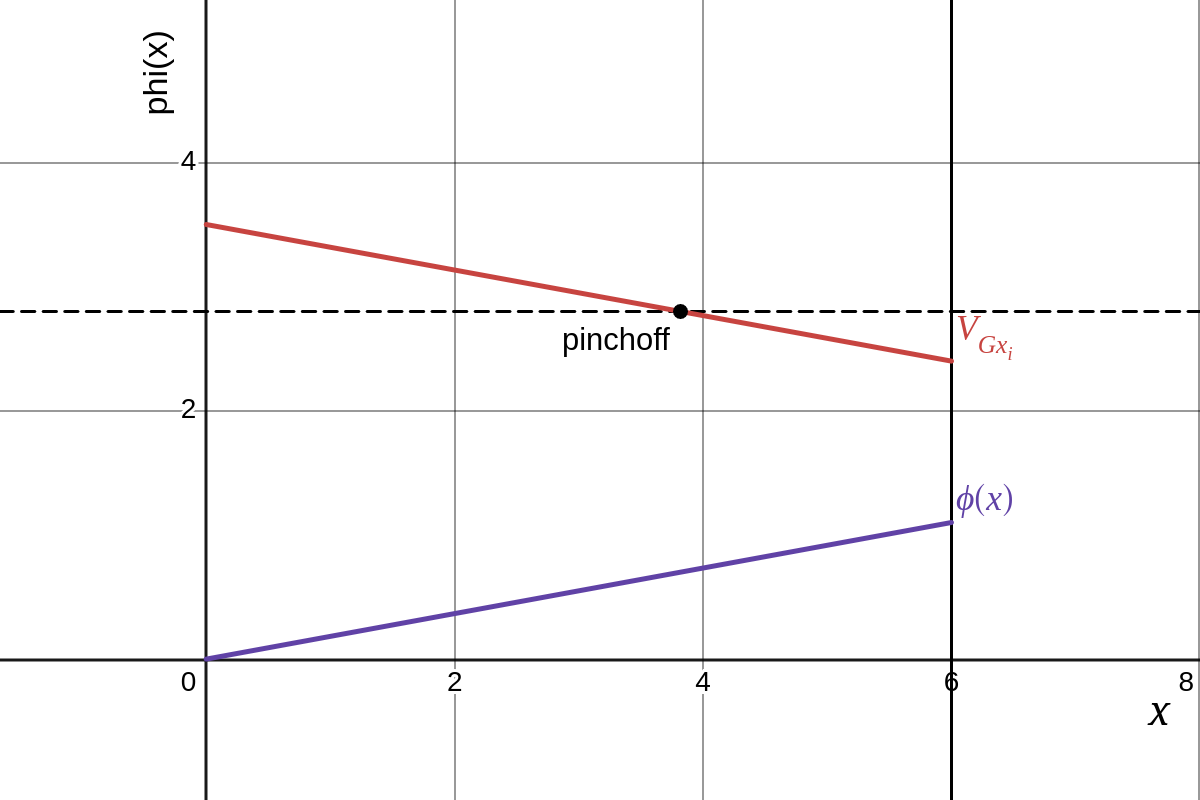
\includegraphics[scale=0.25]{../figures/pinchoff.png}
	\end{center}

Per una $V_D$ al di sopra del punto di pinchoff qualsiasi, in particolare, vale che il canale si chiude all'ascissa:
$$
x_p = \frac{\left(V_{G}-V_{T}\right)L}{V_{D}}
$$
Se questo non fosse immediato dalle formule, una visualizzazione di questa situazione si può trovare qui: \url{https://www.desmos.com/calculator/qhnrqn8kcq}.

Vediamo che la chiusura del canale di conduzione non porta al non passaggio della corrente, ma al fatto che questa diventa costante. Infatti, anche dopo il punto di pinchoff, si ha che la zona del gate lasciata senza elettroni mobili si comporta come una giunzione PN e riesce comunque a condurre corrente. Per capire come mai la corrente resta costante, prendiamo $\Lambda L$ come la lunghezza della giunzione formata:
$$
\Delta L = L - x_p
$$
Quindi descriviamo 3 variabili che restano costanti:
\begin{itemize}
	\item Vediamo che se $\Delta L << L$, la resistenza del canale cambia di poco in quanto:
	$$
	R = \rho \frac{L}{S} \approx \rho \frac{L - \Delta L}{S}
	$$
	dalla seconda legge di Ohm;
	\item La differenza di potenziale fra il punto di pinchoff e il source (preso a riferimento) resterà costante per definizione in quanto $x_p$ viene presa perché sia:
	$$
	\phi(x_p) = V_G - V_T
	$$
	\item Il numero di elettroni liberi nella zona di interdizione dal pinchoff in poi resta pressapoco costante.
\end{itemize}
Da questo deriva il fatto che le caratteristiche della giunzione formata restano costanti al variare di $x_p$ (e quindi di $V_D$ oltre il punto di pinchoff), e quindi lo resta anche la corrente che passa sul MOSFET dal drain al source. Per questo motivo chiamiamo questa zona, di \textbf{saturazione}. 

Notiamo che la saturazione nel MOSFET ha effettivamente un comportamento macroscopico simile a quella del BJT, ma viene provocata da fenomeni completamente diversi all'interno della struttura del transistore

\end{itemize}

\end{itemize}

Abbiamo quindi ricavato una caratteristica per il transistor MOSFET che è effettivamente simile a quella di uscita del BJT (cioè al variare della $V_{CE}$), dove abbiamo:
\begin{enumerate}
	\item Una prima regione \textit{ohimca} dove si comporta come resistenza controllata in tensione;
	\item Una regione intermedia dove il canale di conduzione va a rimpicciolorsi e la relazione diventa non lineare;
	\item Una regione di \textit{saturazione} dove la corrente rimane costante al variare della tensione al drain $V_D$.
\end{enumerate}

\subsection{Modelli per il MOSFET}
Vediamo quale può essere una modellizzazione del MOSFET che ci permette di trattarlo nei circuiti, senza considerare il suo comportamento al livello microscopico.

\begin{enumerate}
	\item \textbf{\textsf{Regione ohmica}} \\
	Quando questo si comporta da \textit{triodo} (cioè è in fase \textbf{ohmica}) abbiamo detto che obbedisce alla legge di Ohm. Sarà allora che la corrente da drain a source vale circa:
	$$
	i_{ds} = \mu_n C_{ox} \frac{W}{L} \left( (V_{GS} - V_T) V_{DS} - \frac{V_{DS}^2}{2} \right) = K \left( (V_{GS} - V_T) V_{DS} - \frac{V_{DS}^2}{2} \right)
	$$
	dove $\mu_n$ è la mobilità elettronica, $W$ è la larghezza del MOSFET, $L$ la lunghezza a cui siamo abituati, e $C_{ox}$ è la capacità dello strato di ossido, data da:
	$$
	C_{ox} = \frac{\text{capacità del gate}}{\text{area}} = \frac{\epsilon_{ox}}{E_{ox}}
	$$

	\item \textbf{\textsf{Regione di saturazione}} \\
	Per il modello in saturazione, dove abbiamo detto la corrente diventa costante, si usa l'approssimazione:
	$$
	i_{ds} = \mu_n C_{ox} \frac{W}{L} \frac{ (V_{GS} - V_T)^2 }{2} = K \frac{(V_{GS} - V_T)^2}{2}
	$$
	che vediamo appunto è costane fissata $V_G$ e calcolata $K$ dagli stessi parametri della regione ohmica.
\end{enumerate}

Per determinare la zona di \textit{transizione} fra regione ohmica e di saturazione, poniamo la condizione di pinchoff:
$$
V_{GS} - V_{DS} = V_T \implies V_{DS} = V_{GS} - V_T
$$

Tracciando l'andamento sul grafico, al variare della $V_{GS}$, si ha:
	\begin{center}
		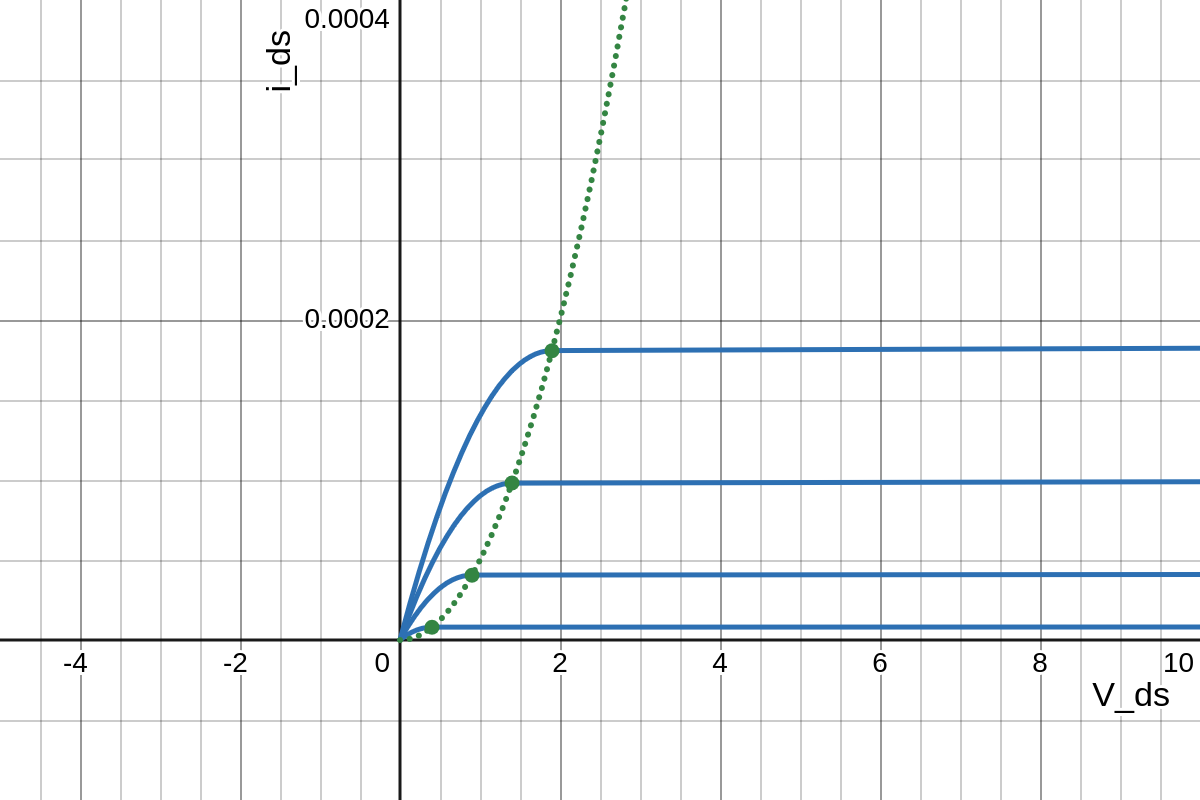
\includegraphics[scale=0.3]{../figures/mosfet_char.png}
	\end{center}
dove si nota la separazione fra regione ohmica (lineare) e di saturazione.

\end{document}
